\documentclass[11pt]{article}

\usepackage[margin=1in]{geometry}
\usepackage[T1]{fontenc}
\usepackage[utf8]{inputenc}
\usepackage{amsmath,amssymb}
\usepackage{booktabs}
\usepackage{array}
\usepackage{threeparttable}
\usepackage{enumitem}
\usepackage{graphicx}
\usepackage[hidelinks]{hyperref}

\setlength{\parindent}{0pt}
\setlength{\parskip}{0.6\baselineskip}
\setlist{nosep,leftmargin=*}

\newcommand{\A}{\text{\AA}}
\setlength{\emergencystretch}{2em}

\title{When Can a Molecular-Dynamics Simulation Stop?\\
\large Toward Anytime-Valid Precision for Equilibrium Observables}
\author{Francisco Hernando-Gallego\textsuperscript{1,*} \quad
Diego Garc\'ia-Santos\textsuperscript{2} \quad
Dimitar Vasilev-Vasilev\textsuperscript{2}\\
Alberto G\'omez-G\'omez\textsuperscript{3} \quad
Alfonso Campo-Camacho\textsuperscript{3}\\[1.2ex]
\small\textsuperscript{1}Department of Applied Mathematics, Escuela de Ingenier\'ia Inform\'atica de Segovia,\\
\small Universidad de Valladolid, 40005 Segovia, Spain\\
\small\textsuperscript{2}Department of Computer Science, Escuela de Ingenier\'ia Inform\'atica de Segovia,\\
\small Universidad de Valladolid, 40005 Segovia, Spain\\
\small\textsuperscript{3}Independent researcher, Spain\\[0.8ex]
\small\textsuperscript{*}Corresponding author: \href{mailto:fhernando@uva.es}{fhernando@uva.es}\\[0.4ex]
\footnotesize ORCID: F.H.-G. \href{https://orcid.org/0000-0003-2995-138X}{0000-0003-2995-138X}; D.G.-S. \href{https://orcid.org/0009-0009-7583-0408}{0009-0009-7583-0408}; D.V.-V. \href{https://orcid.org/0009-0002-3391-5031}{0009-0002-3391-5031};\\
A.G.-G. \href{https://orcid.org/0009-0007-3009-5353}{0009-0007-3009-5353}; A.C.-C. \href{https://orcid.org/0009-0002-2234-4341}{0009-0002-2234-4341}}
\date{}

\begin{document}
\maketitle

\begin{abstract}
Molecular-dynamics (MD) simulations are usually run for a prespecified duration, even when the goal is to estimate an equilibrium observable to a stated precision. Stopping as soon as an estimated uncertainty becomes small enough is attractive, but repeated inspection invalidates uncertainty statements calibrated for a fixed time. We formulate data-dependent stopping as an inferential problem with an explicit precision target and a simultaneous-in-time coverage requirement, and organise it into four gated stages: temporal prediction against strong baselines, uncertainty calibration, an anytime-valid stopping rule, and measured high-performance-computing (HPC) savings. We report exploratory first-stage results on four incrementally assembled ATLAS cohorts, using sequence-grouped cross-validation and a target computed only from frames after a 20~ns prefix. In the largest cohort (757 systems, 1,243 replicas, 689 sequence groups), ridge regression on 48 prefix summaries and a residual gated recurrent unit (GRU) both reduced RMSD mean absolute error relative to last-value persistence (0.610 and 0.636 versus 0.673~\A; paired bootstrap intervals excluding zero), whereas the GRU--ridge difference was not significant in any cohort. A genuine structure-only baseline, a compatible mdCATH analysis, sequential coverage and HPC cost measurements are still outstanding, so no stopping policy or computational saving is claimed.
\end{abstract}

\section{Introduction}

Molecular dynamics is a standard route to protein conformational behaviour, but extracting an equilibrium quantity from a finite trajectory raises two questions: whether the trajectory has sampled enough for the quantity of interest, and whether further simulation is worth its cost. Large standardised trajectory collections such as ATLAS and mdCATH make it possible to study predictive and statistical tools across many proteins and replicas rather than a few hand-selected systems \cite{VanderMeersche2024ATLAS,Mirarchi2024mdCATH}. A model that forecasts the endpoint of a trajectory is not, however, a justified criterion for terminating it.

The question addressed here is: \emph{when may a simulation be stopped if the goal is to estimate an equilibrium observable within tolerance $\varepsilon$ at confidence level $1-\alpha$, and the stopping time may depend on the observed trajectory?} A fixed-horizon prediction interval does not retain its nominal coverage once it has been inspected repeatedly and used to choose when to stop. The objective is therefore not to predict an endpoint or detect a visual plateau, but to construct and test a procedure whose coverage guarantee holds under the adaptive stopping rule that is actually used.

We plan this work in four stages, each with a go/no-go gate:
\begin{enumerate}
\item \textbf{Prediction against strong baselines.} At scale, a temporal predictor must improve on ridge regression over prefix summaries, on a genuine structure-only predictor, and on last-value persistence.
\item \textbf{Uncertainty calibration.} Predictive uncertainty must be quantified and calibrated on held-out systems.
\item \textbf{Anytime-valid stopping.} A sequential interval and stopping rule must be constructed, with its assumptions stated and its coverage checked under the rule's own stopping behaviour.
\item \textbf{Measured savings.} The rule must be benchmarked on the SCAYLE HPC system, measuring realised core-hours including all overheads.
\end{enumerate}

This preprint contributes the formal statement of the problem (Section~\ref{sec:problem}), the evaluation protocol and gate for Stage~1 (Section~\ref{sec:methods}), and exploratory Stage~1 results on ATLAS cohorts of 80 to 942 systems (Section~\ref{sec:results}). The work builds on an earlier study of temporal surrogates on 20 ATLAS proteins, including a GRU configured by an Improved Grey Wolf Optimizer \cite{HernandoGallego2026Mathematics}, in which last-value persistence had the lowest nominal error for all five observables and ridge regression was competitive. We therefore treat persistence and ridge as substantive controls, not straw baselines, and hyperparameter metaheuristics are not a contribution of this work.

The claims are deliberately limited. The Stage~1 gate (Milestone~0) has not been passed, because the structure-only baseline and the mdCATH analysis are still missing; held-out validation and test predictions have not been evaluated; and no anytime-valid coverage or simulation saving is claimed.

\section{Problem formulation}\label{sec:problem}

Let $X_{i,r}(u)$ be the trajectory state of system $i$, replica $r$, at simulation time $u$. For an observable $g$, the physical estimand $\Theta_{i,g}$ is its equilibrium expectation under the specified ensemble and simulation conditions. It is distinct from the finite-trajectory label $Y_{i,r,g}$, computed from the accepted post-equilibration window of replica $r$, which is only an operational reference for $\Theta_{i,g}$.

At inspection time $t$, let $\mathcal{F}_{i,r,t}$ contain the observed prefix up to $t$ together with any permitted static inputs and prespecified metadata, and let $C_{i,r,g,t}$ be an interval for $\Theta_{i,g}$ built from $\mathcal{F}_{i,r,t}$. For a target-specific tolerance $\varepsilon_g>0$, the stopping time is
\[
  \tau_{i,r,g}=\inf\{t\in\mathcal{T}_g: \operatorname{width}(C_{i,r,g,t})\leq 2\varepsilon_g\},
\]
and the required property is simultaneous coverage over the inspection grid $\mathcal{T}_g$:
\begin{equation}
  \Pr_{\mathrm{MD,cal}}\!\left(\forall t\in\mathcal{T}_g,\;\Theta_{i,g}\in C_{i,r,g,t}
  \middle| i,g,\mathcal{E},\mathcal{P}\right)\geq 1-\alpha_g.
  \label{eq:anytime}
\end{equation}
Here $\mathcal{E}$ denotes the ensemble and force-field conditions and $\mathcal{P}$ the simulation protocol. The probability is over MD trajectories generated under the protocol (including randomised initial conditions) and over the calibration data, conditional on the system, observable, ensemble, force field and protocol. If Equation~\eqref{eq:anytime} holds under stated assumptions, coverage also holds at the data-dependent time $\tau_{i,r,g}$; a fixed-horizon calibrated interval does not provide this. Two points remain open and are part of the programme: the assumptions under which Equation~\eqref{eq:anytime} can be established, and the reference needed to assess coverage of $\Theta_{i,g}$, since empirical coverage measured against $Y_{i,r,g}$ concerns only that finite-trajectory reference.

\section{Data and methods}\label{sec:methods}

\subsection{Trajectories, inputs and targets}

All experiments use ATLAS, which provides three 100~ns replicas per protein chain \cite{VanderMeersche2024ATLAS}. The model input is the 0--20~ns prefix sampled every 100~ps (201 points) with eight channels: backbone RMSD to the first frame (\A); mass-weighted radius of gyration $R_g$ (\A); replica-specific core RMSDs at the 30th, 40th and 50th C$\alpha$-RMSF quantiles (\A), where cores are low-RMSF residues computed from that replica's prefix only, with segments shorter than three residues removed; total Shrake--Rupley SASA (\A$^2$); and simplified-DSSP helix and strand fractions \cite{Kabsch1983DSSP}. Inputs are raw physical values; scaling is fitted within each training partition.

Equilibration is detected per observable with the Chodera/\allowbreak PyMBAR procedure, and the autocorrelation-corrected effective sample size $N_{\mathrm{eff}}=N/g$ is computed for the accepted window \cite{Chodera2016Equilibration}. For replica $r$ of system $i$, with $x_{i,r,g,j}$ the observable at sampled frame $j$, $j_{0,i,r,g}$ the first accepted frame and $J$ the final frame, the label is the mean over the accepted window,
\begin{equation}
  Y_{i,r,g} = \frac{1}{J-j_{0,i,r,g}+1}\sum_{j=j_{0,i,r,g}}^{J}x_{i,r,g,j}.
  \label{eq:target-mean}
\end{equation}
A label is valid only when the accepted window lasts at least 20~ns and $N_{\mathrm{eff}}\geq 10$; invalid labels are masked, not imputed. Two target definitions are used:
\begin{itemize}
\item \textbf{Original target.} The accepted window starts at the detected equilibration time $t_0$, which may fall inside the 0--20~ns prefix. This is the definition of the earlier study and of the historical 80-system analyses (Section~\ref{sec:atlas80}).
\item \textbf{Future-only target.} The window uses only frames with $t>20$~ns and $t\geq t_0$, so the label never shares frames with the input. Duration, $N_{\mathrm{eff}}$ and validity are recomputed on this window. All scaled cohorts use this definition, for RMSD only.
\end{itemize}

\subsection{Cohorts and partitions}

Cohorts were assembled incrementally from ATLAS (Table~\ref{tab:cohorts}); they overlap and are not independent samples. Sequence groups are connected components of pairwise BLAST links with at least 30\% identity and at least 80\% coverage of both sequences, plus links for identical sequences and for chains sharing a PDB identifier. Grouping prevents near-identical sequences from being split across folds but does not exclude remote homology.

The historical 80-system split is frozen at 62 training, 9 validation and 9 test systems, and every later cohort keeps those assignments and adds new systems to training. All results below are cross-validation on training systems. The nine validation systems were inspected during development of the 80-system pilot, so they are not an untouched validation set. No test-set predictions or errors have been computed for any cohort. A retrospective audit of target-window metadata for the 80-system pilot did include the test systems (Section~\ref{sec:atlas80}); those metadata were not used to select models, thresholds or exclusions.

One system (\texttt{3txs\_C}) was excluded from the 222-system assembly because its prefix core at the 30th quantile was empty; the decision was made during processing and was not preregistered.

\begin{table}[ht]
\centering
\small
\begin{threeparttable}
\caption{Cohorts. Assembled counts refer to the whole cohort; evaluated counts are the training systems with at least one valid future-only RMSD label.}
\label{tab:cohorts}
\begin{tabular}{lrrrrrrr}
\toprule
 & \multicolumn{3}{c}{Assembled} & & \multicolumn{3}{c}{Evaluated in CV} \\
\cmidrule{2-4}\cmidrule{6-8}
Cohort & Systems & Replicas & Groups & Train & Systems & Replicas & Groups \\
\midrule
ATLAS80\tnote{a}  & 80  & 240   & --- & 62  & 53  & 92    & ---\\
ATLAS222 & 222 & 666   & 191 & 204 & 170 & 288   & 149 \\
ATLAS362 & 362 & 1,086 & 318 & 344 & 286 & 477   & 258 \\
ATLAS742 & 742 & 2,226 & 660 & 724 & 596 & 988   & 541 \\
ATLAS942 & 942 & 2,826 & 835 & 924 & 757 & 1,243 & 689 \\
\bottomrule
\end{tabular}
\begin{tablenotes}[flushleft]
\footnotesize
\item[a] Historical pilot, grouped by protein rather than by sequence group; 93 replicas are valid under the original target and 92 under both definitions.
\end{tablenotes}
\end{threeparttable}
\end{table}

\subsection{Models}

All models predict the system-level future-only RMSD label from the 0--20~ns prefix.
\begin{itemize}
\item \textbf{Trained mean}: the mean label of the training partition.
\item \textbf{Last-value persistence}: the last observed RMSD of the prefix.
\item \textbf{First-frame ridge} (\texttt{snapshot0\_ridge}): ridge regression on $R_g$, SASA, helix and strand at the first frame. Because these are trajectory-derived values, it is \emph{not} the structure-only baseline required by Milestone~0; it is reported only as an exploratory control.
\item \textbf{Ridge}: ridge regression on 48 prefix summaries (mean, population standard deviation, minimum, maximum, last value and linear slope against time rescaled to $[-1,1]$ for each of the eight channels), with $\alpha\in\{0.01,0.1,1,10,100\}$ selected by four inner folds grouped by sequence group.
\item \textbf{Residual GRU}: a one-layer GRU with 32 hidden units and a zero-initialised linear head that predicts a correction to the last observed RMSD, so that at epoch zero it reproduces persistence. It is trained with Adam (learning rate $10^{-3}$, weight decay $10^{-4}$, at most 150 epochs), and the number of epochs is selected on an internal hold-out of about 20\% of the groups in each outer training partition, with patience 20.
\end{itemize}

\subsection{Evaluation}

Each scaled cohort uses five outer folds with sequence groups disjoint across folds; hyperparameters are selected inside each outer training partition. Models are fitted with equal weight per valid replica; for evaluation, predictions and labels are averaged over the valid replicas of each system, so each system has equal weight. We report out-of-fold mean absolute error (MAE), root-mean-square error (RMSE) and $R^2$. Paired differences in MAE carry percentile 95\% intervals from 10,000 bootstrap resamples of complete sequence groups, using the same resamples for every model.

These intervals are conditional on the fitted out-of-fold predictions: they do not repeat model training or selection, and they do not adjust for the repeated exploratory decisions made while the pipeline was developed. They should be read as descriptive measures of uncertainty, not as confirmatory tests.

\subsection{Milestone~0: the Stage~1 gate}

Milestone~0 must be passed before a stopping policy is developed. On a large ATLAS cohort and a compatible mdCATH subset, the temporal predictor must outperform both (i) ridge regression on the 48 prefix summaries and (ii) a genuine predictor using static structure alone, by MAE aggregated per protein, with last-value persistence as an additional control. The quantitative threshold and the rule for aggregating across cohorts will be fixed before validation or test predictions are evaluated.

\section{Results}\label{sec:results}

\subsection{Scaled cohorts with a future-only RMSD target}\label{sec:scaled}

Table~\ref{tab:scaled} summarises the four scaled cohorts and Figure~\ref{fig:contrasts} shows the paired contrasts. Three patterns are consistent across cohorts.

\emph{Observing the prefix helps.} The first-frame ridge control is far worse than every prefix-based model (MAE 1.69--1.89~\A\ against 0.61--0.79~\A), so most of the predictive information comes from the observed prefix rather than from the initial conformation alone.

\emph{Both prefix models beat persistence as the cohort grows.} The GRU--persistence interval excludes zero in ATLAS362, ATLAS742 and ATLAS942, and the ridge--persistence interval excludes zero in ATLAS942. In the largest cohort, ridge reduces MAE by 9.4\% relative to persistence and the GRU by 5.5\%. This contrasts with the 20-protein study, where persistence had the lowest nominal error \cite{HernandoGallego2026Mathematics}.

\emph{The GRU does not outperform ridge.} The GRU had the lowest point MAE in ATLAS222, ATLAS362 and ATLAS742, and ridge in ATLAS942, but the GRU--ridge interval includes zero in all four cohorts. Ridge has equal or better RMSE and $R^2$ in ATLAS362, ATLAS742 and ATLAS942. Recurrent modelling has therefore not shown an advantage over a regularised linear model of prefix summaries.

The four cohorts overlap and their evaluated populations and folds differ, so the decreasing point MAE from ATLAS362 to ATLAS942 is not a learning curve. Ridge selected the upper end of its penalty grid ($\alpha=100$) in 2, 5 and 4 of the five folds in ATLAS222, ATLAS742 and ATLAS942; the grid will be extended before the protocol is frozen.

\begin{table}[ht]
\centering
\small
\caption{Out-of-fold RMSD prediction with a future-only target, by cohort. System-level metrics; MAE and RMSE in \A.}
\label{tab:scaled}
\footnotesize
\setlength{\tabcolsep}{4pt}
\begin{tabular}{lrrrrrrrrr}
\toprule
 & \multicolumn{3}{c}{ATLAS222} & \multicolumn{2}{c}{ATLAS362} & \multicolumn{2}{c}{ATLAS742} & \multicolumn{2}{c}{ATLAS942}\\
\cmidrule(lr){2-4}\cmidrule(lr){5-6}\cmidrule(lr){7-8}\cmidrule(lr){9-10}
Model & MAE & RMSE & $R^2$ & MAE & $R^2$ & MAE & $R^2$ & MAE & $R^2$ \\
\midrule
Trained mean          & 2.227 & 3.126 & $-0.008$ & 2.349 & $-0.012$ & 2.085 & $-0.002$ & 1.988 & $-0.004$ \\
Persistence           & 0.729 & 1.267 & 0.834 & 0.791 & 0.826 & 0.690 & 0.834 & 0.673 & 0.830 \\
First-frame ridge     & 1.756 & 2.415 & 0.399 & 1.891 & 0.287 & 1.732 & 0.244 & 1.691 & 0.202 \\
Ridge, 48 summaries   & 0.787 & 1.228 & 0.845 & 0.772 & 0.852 & 0.655 & 0.857 & \textbf{0.610} & \textbf{0.870} \\
Residual GRU          & \textbf{0.703} & \textbf{1.226} & \textbf{0.845} & \textbf{0.752} & 0.852 & \textbf{0.641} & 0.852 & 0.636 & 0.848 \\
\bottomrule
\end{tabular}

\vspace{1ex}
\begin{tabular}{lrrrr}
\toprule
RMSE (\A) & ATLAS222 & ATLAS362 & ATLAS742 & ATLAS942 \\
\midrule
Persistence & 1.267 & 1.338 & 1.193 & 1.183 \\
Ridge, 48 summaries & 1.228 & \textbf{1.235} & \textbf{1.104} & \textbf{1.034} \\
Residual GRU & \textbf{1.226} & 1.236 & 1.125 & 1.116 \\
\bottomrule
\end{tabular}
\end{table}

\begin{figure}[ht]
\centering
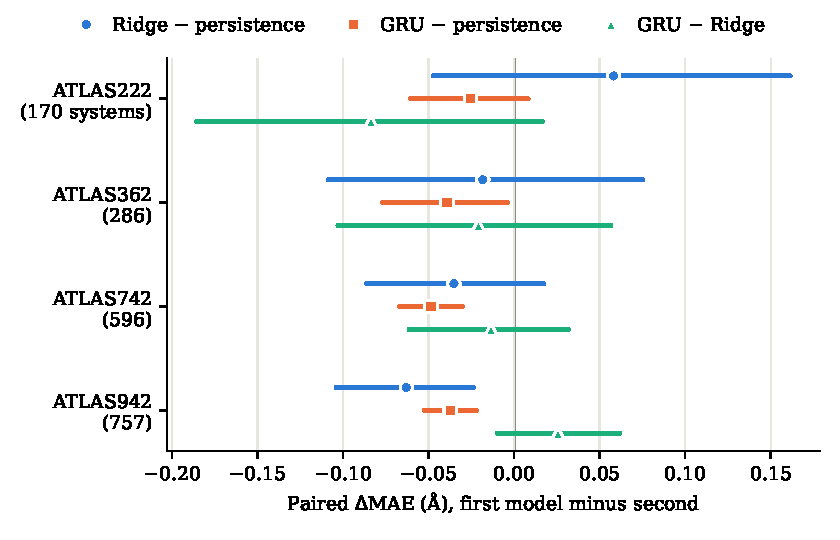
\includegraphics[width=0.82\linewidth]{figures/fig1_paired_contrasts.pdf}
\caption{Paired differences in system-level MAE (first model minus second; negative values favour the first model), with 95\% group-bootstrap intervals, for the four scaled cohorts. Numbers in parentheses are evaluated systems. Values are listed in Table~\ref{tab:contrasts}.}
\label{fig:contrasts}
\end{figure}

\begin{table}[ht]
\centering
\small
\caption{Paired MAE differences in \A\ with 95\% group-bootstrap intervals (first model minus second).}
\label{tab:contrasts}
\begin{tabular}{lccc}
\toprule
Cohort & Ridge $-$ persistence & GRU $-$ persistence & GRU $-$ Ridge \\
\midrule
ATLAS222 & $+0.058$ [$-0.047$, $+0.161$] & $-0.025$ [$-0.060$, $+0.008$] & $-0.084$ [$-0.186$, $+0.016$] \\
ATLAS362 & $-0.018$ [$-0.108$, $+0.075$] & $-0.039$ [$-0.077$, $-0.004$] & $-0.021$ [$-0.103$, $+0.057$] \\
ATLAS742 & $-0.035$ [$-0.086$, $+0.017$] & $-0.049$ [$-0.067$, $-0.030$] & $-0.013$ [$-0.061$, $+0.032$] \\
ATLAS942 & $-0.063$ [$-0.104$, $-0.024$] & $-0.037$ [$-0.052$, $-0.022$] & $+0.026$ [$-0.010$, $+0.062$] \\
\bottomrule
\end{tabular}
\end{table}

In ATLAS222, two folds selected epoch zero for the GRU, which then reproduces persistence; this explains the 68 systems on which GRU and persistence tie. Fold-wise hyperparameter selections are listed in Appendix~\ref{app:provenance}.

\subsection{Historical 80-system pilot}\label{sec:atlas80}

The 80-system pilot preceded the future-only target and used the original target definition, with folds grouped by protein. Under that definition, the 0--20~ns prefix and the target window can share frames. A retrospective audit found positive overlap in 130 of the 691 valid replica--target labels (18.8\%; 17.4\% for RMSD, 29.5\% for $R_g$, 28.1\% for SASA and 12.5\% for each secondary-structure fraction). This is overlap within a trajectory, not leakage between proteins, but it means the original target is not a strictly future prediction. It motivated the future-only definition used above.

Table~\ref{tab:atlas80} reports the pilot's RMSD cross-validation on 53 training proteins, first with the original target and then retrained on the 92 replicas that are valid under both definitions. Ridge and the GRU have lower point MAE than persistence in all three settings, but the GRU--ridge difference is never significant:
\begin{itemize}
\item \textbf{Original target} (93 replicas): GRU $-$ ridge $-0.012$~\A\ [$-0.120$, $+0.102$], with 26 of 53 proteins favouring the GRU; GRU $-$ persistence $-0.100$~\A\ [$-0.160$, $-0.037$]; ridge $-$ persistence $-0.088$~\A\ [$-0.208$, $+0.026$].
\item \textbf{Common mask, future-only target} (92 replicas): GRU $-$ ridge $-0.010$~\A\ [$-0.152$, $+0.163$]; GRU $-$ persistence $-0.103$~\A\ [$-0.164$, $-0.040$].
\end{itemize}
Moving from the original to the future-only target left the GRU unchanged (difference $<0.002$~\A) and lowered ridge MAE by 0.042~\A\ [$-0.090$, $-0.003$]. Almost all of that change came from a single fold of 11 proteins, where ridge selected a different penalty under each definition; with the penalty held fixed, the two definitions differed by less than 0.003~\A\ in that fold. The apparent narrowing of the GRU's advantage therefore reflects model selection rather than a demonstrated effect of overlap. On the seven validation proteins, which were inspected during development, MAE was 0.714~\A\ for ridge, 0.784~\A\ for the GRU and 0.969~\A\ for persistence.

\begin{table}[ht]
\centering
\small
\caption{Historical 80-system pilot: five-fold, protein-grouped RMSD cross-validation on 53 training proteins (protein-level metrics; MAE and RMSE in \A).}
\label{tab:atlas80}
\begin{tabular}{lrrrrrrrrr}
\toprule
 & \multicolumn{3}{c}{Original target, 93 replicas} & \multicolumn{3}{c}{Original, common mask} & \multicolumn{3}{c}{Future-only, common mask} \\
\cmidrule(lr){2-4}\cmidrule(lr){5-7}\cmidrule(lr){8-10}
Model & MAE & RMSE & $R^2$ & MAE & RMSE & $R^2$ & MAE & RMSE & $R^2$ \\
\midrule
Persistence & 0.566 & 0.830 & 0.659 & 0.627 & 1.110 & 0.555 & 0.628 & 1.111 & 0.555 \\
Ridge       & 0.478 & 0.689 & 0.765 & 0.577 & 0.846 & 0.742 & 0.535 & 0.818 & 0.759 \\
GRU         & 0.466 & 0.762 & 0.712 & 0.525 & 1.059 & 0.596 & 0.525 & 1.059 & 0.595 \\
\bottomrule
\end{tabular}
\end{table}

\subsection{Status of Milestone~0}

Milestone~0 has not been passed. The results support a forecasting signal in the 20~ns prefix that transfers to unseen sequence groups and exceeds persistence at scale. They do not show that a recurrent model adds information beyond ridge regression, and they cannot yet be attributed to dynamics rather than structure, because the required structure-only baseline and the mdCATH analysis are still missing.

\section{Planned stages}

\textbf{Completing Stage~1.} Implement a predictor whose inputs are genuinely static structural information, with no trajectory-derived observables; select an mdCATH subset in which each domain is grouped across temperatures; run homology-aware sensitivity analyses of the sequence grouping; extend the ridge penalty grid; and fix the observables, baselines, quantitative threshold and selection protocol before any validation or test prediction is evaluated.

\textbf{Stage~2: uncertainty calibration.} Compare calibration procedures on held-out systems, stratified by target, trajectory length and system characteristics. The analysis must state whether coverage refers to the replica label $Y_{i,r,g}$ or to the system-level estimand $\Theta_{i,g}$ after a prespecified aggregation of replicas, and account for replica and protein dependence. Calibration at a fixed horizon is not evidence of coverage under data-dependent stopping.

\textbf{Stage~3: anytime-valid stopping.} Construct a sequential interval procedure, state sufficient assumptions for Equation~\eqref{eq:anytime} or an explicitly justified alternative, and evaluate coverage and achieved precision at the actual adaptive stopping time. Comparators are fixed-horizon stopping, prespecified plateau heuristics, and classical equilibration and correlated-sample methods; the Chodera/PyMBAR procedure is used to build targets and is not presumed to solve the stopping problem.

\textbf{Stage~4: measured savings.} Run the frozen stopping rule and its comparators on SCAYLE, pairing or randomising trajectories and run allocations, and report wall-clock time and core-hours including online analysis, inference, checkpoints and scheduling overheads, alongside the achieved error and coverage.

\section{Discussion}

The main empirical result is that a 20~ns prefix carries information about the future-only mean RMSD that transfers to unseen sequence groups and, at the scale of several hundred systems, improves on persistence. This is the precondition for the rest of the programme, not a solution to it, and three limitations govern its interpretation.

First, the structure-only baseline is decisive. First-frame trajectory descriptors are not a static structure-only comparator, so the gain over persistence cannot yet be attributed to dynamic information beyond what the structure already encodes. The sequence grouping excludes near-identical sequences across folds but not remote homology, and the group bootstrap does not capture variability from model fitting, selection or repeated exploratory decisions.

Second, prediction is not inference. Even an accurate predictor with an interval calibrated at a fixed horizon loses that calibration when it is monitored repeatedly and used to decide when to stop. A valid procedure must address the whole monitoring process, with an explicit estimand, inspection schedule, calibration strategy, dependence assumptions and stopping rule. These are obligations of design and proof, not implementation details.

Third, simulated time is not a proxy for HPC savings. Online analysis consumes resources, jobs carry fixed overheads, and early stopping may change utilisation and scheduling. Savings must be measured in a controlled campaign, and the prefix analyses reported here are not evidence of them.

The comparison between ridge and the GRU also has a practical implication: until a temporal architecture beats a regularised linear model of prefix summaries under the frozen protocol, the simpler model should be preferred for the calibration and stopping stages.

\section{Conclusion}

We have formulated the stopping of MD simulations as an anytime-valid inference problem and organised its solution into four gated stages. Exploratory Stage~1 results on ATLAS cohorts of up to 757 evaluated systems show that ridge regression and a residual GRU on a 20~ns prefix both predict the future-only mean RMSD better than persistence, while neither outperforms the other. Milestone~0 remains open until a genuine structure-only baseline and a compatible mdCATH analysis are in place; sequential coverage, stopping-policy experiments and HPC cost measurements follow. No anytime-valid coverage, general model superiority or measured simulation saving is claimed.

\section*{Data and code availability}
ATLAS trajectories are publicly available from their authors under a CC BY-NC 4.0 licence \cite{VanderMeersche2024ATLAS}; no trajectories are redistributed here. The manuscript source, the cohort-level metrics and paired contrasts behind Tables~\ref{tab:scaled}--\ref{tab:contrasts} and Figure~\ref{fig:contrasts}, the script that draws the figure, and a snapshot of the training and evaluation code are available at \url{https://github.com/fhernandogallego/md-anytime-stopping}. The full evidence bundles for each cohort, including fold manifests and prediction files, are archived at pinned commits in \url{https://github.com/fhernandogallego/md-hpc-benchmarks-public} and identified by the SHA-256 digests in Appendix~\ref{app:provenance}.

\section*{Author contributions}
Conceptualization, F.H.-G. and A.C.-C.; methodology, F.H.-G., D.G.-S. and D.V.-V.; software, D.G.-S. and D.V.-V.; validation, D.V.-V., D.G.-S. and A.G.-G.; formal analysis, F.H.-G. and D.V.-V.; investigation, D.G.-S. and D.V.-V.; data curation, D.G.-S.; writing---original draft, F.H.-G. and D.G.-S.; writing---review and editing, A.C.-C., A.G.-G. and F.H.-G.; visualization, D.V.-V. and D.G.-S.; supervision, A.C.-C.; project administration, F.H.-G. and A.G.-G. All authors have read and agreed to this version of the manuscript.

\section*{Funding}
This research received no external funding.

\section*{Competing interests}
F.H.-G. holds equity in Fransdata Tech Ventures S.L., a company with which A.G.-G. and A.C.-C. are also associated. The company did not fund this work, and no commercial use of ATLAS data is made.

\section*{Acknowledgments}
Computations were performed at the SCAYLE supercomputing centre (Castilla y Le\'on, Spain).

\bibliographystyle{plain}
\bibliography{references}

\appendix
\section{Provenance and reproducibility}\label{app:provenance}
\small\sloppy

SHA-256 digests are shown in groups of eight characters, which concatenate without separators.

\textbf{Splits and datasets.}
\begin{itemize}
\item Frozen 80-system split: \texttt{d31ef5c7\allowbreak d5fcea49\allowbreak e4f6414e\allowbreak a8bb7025\allowbreak 4ee5c630\allowbreak 08b8c027\allowbreak 07ab462c\allowbreak 31e24bee}.
\item ATLAS222 assembled dataset: \texttt{ea2e00c4\allowbreak a542c8e9\allowbreak 5ca155be\allowbreak 58e5e36e\allowbreak 70f2985b\allowbreak 220f83cf\allowbreak 2cb25211\allowbreak 68ae4058}.
\item Audited 80-system target-window metadata (audit of 8 October 2026): \texttt{1899e312\allowbreak 1864ced9\allowbreak e7b50bcf\allowbreak 9a4ee5f7\allowbreak bd761420\allowbreak 2af035a7\allowbreak f9a45cd4\allowbreak 42ad6181}.
\end{itemize}

\textbf{Predictions.}
\begin{itemize}
\item ATLAS222 system-level predictions: \texttt{5fdc78cf\allowbreak e10b5f63\allowbreak 9e74d406\allowbreak 0ae34d4a\allowbreak 54da523b\allowbreak ee9cd227\allowbreak 8a7879aa\allowbreak 23a475f9}; outer-fold manifest: \texttt{a4508865\allowbreak 46d0b9ed\allowbreak 2a3ed7e3\allowbreak 77b31da4\allowbreak 5af21270\allowbreak 70651ab9\allowbreak df61aa4f\allowbreak ea3b9d38}. Slurm runs 3239212 (CV), 3239213 (aggregation) and 3239232 (audit).
\item ATLAS742 predictions: \texttt{a4249df4\allowbreak 762b16cc\allowbreak f7b2004e\allowbreak 130923b4\allowbreak 1bc8d2c1\allowbreak 21dd12b4\allowbreak 0e49a22e\allowbreak d89c909f}. Slurm controller 3256792.
\item ATLAS942 predictions: \texttt{a765eb94\allowbreak 0c6d61d0\allowbreak 1774a911\allowbreak b5cdaa63\allowbreak 0b3a7376\allowbreak 693af114\allowbreak 594a2b16\allowbreak 8e12fe7f}. Slurm controller 3262490; evidence bundle of 272 files.
\end{itemize}

\textbf{Public results reports.} ATLAS362: \href{https://github.com/fhernandogallego/md-hpc-benchmarks-public/tree/paper2-atlas362-results-20261020/reports/paper2_atlas362_cv_20261020}{branch \texttt{paper2-atlas362-results-20261020}}. ATLAS942: \href{https://github.com/fhernandogallego/md-hpc-benchmarks-public/tree/paper2-atlas942-results-20261103/reports/paper2_atlas942_cv_20261103}{branch \texttt{paper2-atlas942-results-20261103}}, commit \texttt{aeac5689\allowbreak 1e06bb00\allowbreak 2d50ebdd\allowbreak 3a1068c8\allowbreak 4fd2c600}. They contain results, code and metadata, not model weights or trajectories.

\textbf{Fold-wise hyperparameters} (folds 0--4).
\begin{itemize}
\item ATLAS222: ridge $\alpha=[10,10,10,100,100]$; GRU epochs $[12,0,15,55,0]$.
\item ATLAS742: ridge $\alpha=100$ in all folds; GRU epochs $[25,19,19,25,25]$.
\item ATLAS942: ridge $\alpha=[10,100,100,100,100]$; GRU epochs $[24,10,21,29,16]$.
\item 80-system common mask: ridge $\alpha=[10,100,100,10,100]$ (original) and $[100,100,100,10,100]$ (future-only); GRU epochs $[30,36,27,29,39]$ under both.
\end{itemize}
Full-training refits (seed 20271007) are retained as research candidates and are distinct from the fold-specific models behind the reported metrics; no performance is claimed for them.

\textbf{Bootstrap seeds.} 20261008 (80-system pilot) and 20261016 (ATLAS222).

\textbf{Related experiment not pooled here.} A separate experiment on 500 ATLAS chains predicted late-window RMSD and $R_g$ means with gradient boosting under a different target definition and different metrics. It reuses systems from the same cohort, so it is not an independent replication, and its results are not combined with those reported here.

\end{document}
